\documentclass[12pt]{beamer}
\usetheme{Boadilla}
\usepackage{booktabs}
\usepackage{enumitem}
\usepackage{tikz}

\newcommand{\E}{\mathbb{E}}
\usefonttheme{professionalfonts}
\usepackage{pgfplots}
\renewcommand{\arraystretch}{1.25}
\usetikzlibrary{trees}
\title[ECON2843]{Lecture 10}
\subtitle{Part 2 Probability and Distributions}
\date{}
\usepackage{amsmath,amssymb,mathtools,wasysym}
\begin{document}
	\begin{frame}
		\titlepage
	\end{frame}
\begin{frame}{Before We Start}
\begin{itemize}
\item[\color{blue}$\blacktriangleright$] So far, we have learned a lot about the principles of probability and distribution.

\begin{itemize}
\item[\color{blue}$\blacktriangleright$] My question is: if you flip a {\bf fair} coin 1000 times, according to the Law of Large Numbers we introduced, you should theoretically get around 500 heads.
\item[\color{blue}$\blacktriangleright$] However, let's say in reality, after many flips, for example, after flipping 800 or 900 times, luck hasn't been on your side and most of the results are heads.
\item[\color{blue}$\blacktriangleright$] In this case, what do you think is the probability of getting heads on your next flip? 
\end{itemize}
\end{itemize}
\end{frame}
\begin{frame}{Before We Start}
	\begin{itemize}
\item[\color{blue}$\blacktriangleright$] According to the Law of Large Numbers, is the next flip more likely to be tails, i.e., with a probability greater than 0.5?
\begin{itemize}
\item[\color{blue}$\blacktriangleright$] Because the Law of Large Numbers tells us that over many trials, the overall relative frequency of heads should be 0.5.
\end{itemize}
\item[\color{blue}$\blacktriangleright$] The above statement is not correct.
\begin{itemize}
	\item[\color{blue}$\blacktriangleright$] Based on what we’ve learned, since each flip is independent of the others, for a fair coin, the probability of heads coming up is always 0.5, regardless of when you flip it.
	\item[\color{blue}$\blacktriangleright$] For repeated independent trials, past results do not affect future outcomes. 
	\item[\color{blue}$\blacktriangleright$] This means that if you lose several gambling games in a row, it does not imply that your chances of winning in the next game are higher.
\end{itemize}
\end{itemize}
\end{frame}
\begin{frame}{Before We Start}
\begin{itemize}
	\item[\color{blue}$\blacktriangleright$] Does this contradict the Law of Large Numbers? No, it doesn’t.
	\begin{itemize}
	\item[\color{blue}$\blacktriangleright$] The Law of Large Numbers tells us that the overall probability of heads will approach 0.5, but extreme cases with low probability, such as many consecutive heads for this case, are still possible; it’s just that the likelihood of such an event occurring is relatively low!
\end{itemize}
\end{itemize}
\end{frame}
	\begin{frame}
We have talked about population distribution, let's talk about sampling distribution today.
\end{frame}

\begin{frame}
	\frametitle{Statistical Inference}
	
	\begin{itemize}[label={\color{blue}$\blacktriangleright$}]
		\item \textbf{Statistical inference:} Determining the behaviour of a population by studying a sample from that population.
		\begin{itemize}[label={\color{blue}$\blacktriangleright$}]
			\item Population parameters describe populations, e.g., population mean $\mu$ and population variance $\sigma^2$.
			\item Population parameters usually unknown.
			\item To find out more about them, we take a random sample of data.
			\item Calculate statistics from sample, e.g., sample mean $\bar{X}$ and sample variance $s^2$.
			\item Use $\bar{X}$ and $s^2$ to estimate $\mu$ and $\sigma^2$.
		\end{itemize}
	\end{itemize}
	
\end{frame}

\begin{frame}
	\frametitle{Statistical Inference}
	
	\begin{itemize}[label={\color{blue}$\blacktriangleright$}]
		\item So we use sample statistics to make inferences about population parameters.
		\item Suppose we take a new sample.
		\item We would probably get a different $\bar{X}$ and $s^2$.
		\item Sample statistics are random variables, so there is variability associated with them.
		\item We would like to know how they differ from sample to sample.
	\end{itemize}
	
\end{frame}

\begin{frame}
	\frametitle{Sampling Distribution}
	
	\begin{itemize}[label={\color{blue}$\blacktriangleright$}]
		\item {\bf Sampling distribution:} The distribution of a sample statistic that would arise if we were to repeatedly take random samples from a population.
		\item {\color{red}Knowing the sampling distribution of a sample statistic can tell us how accurately we are estimating a population parameter.}
		\item We will focus on the sampling distribution of the sample mean and the sampling distribution of the sample proportion.
	\end{itemize}
	
\end{frame}

\begin{frame}
	\frametitle{Example 1}
	
	\begin{itemize}[label={\color{blue}$\blacktriangleright$}]
		\item Suppose we roll a fair four-sided die and let $X$ be the number that comes up.
		\item The population can be thought of as an infinite number of rolls of the die.
		\item Let's repeatedly draw samples of size 2, i.e., roll the die twice.
		\item Find the sampling distribution of the sample mean $\bar{X}$.
	\end{itemize}
	
\end{frame}
\begin{frame}
	\frametitle{Probability Distribution of $X$}
	\begin{center}
	\begin{tabular}{ccccc}
		\toprule
		$x$&$1$&$2$&$3$&$4$\\
		\midrule
		$p(x)$&$\frac{1}{4}$&$\frac{1}{4}$&$\frac{1}{4}$&$\frac{1}{4}$\\
		\bottomrule
	\end{tabular}
\end{center}
\begin{itemize}[label={\color{blue}$\blacktriangleright$}]
	\item Remember that probability distributions represent populations.
	\item We can calculate the population mean and population variance from the probability distribution in the usual way.
\end{itemize}
\end{frame}

\begin{frame}
	\frametitle{Mean and Variance of $X$}
	\begin{center}
		\begin{tabular}{ccccc}
			\toprule
			$x$&$1$&$2$&$3$&$4$\\
			\midrule
			$p(x)$&$\frac{1}{4}$&$\frac{1}{4}$&$\frac{1}{4}$&$\frac{1}{4}$\\
			\bottomrule
		\end{tabular}
	\end{center}
	$$\mu=E(X)=\sum_{\text{all }x}(x\times p(x))=\frac{5}{2}$$
	$$\sigma^2=V(X)=E(X^2)-(E(X))^2=\frac{15}{2}-(\frac{5}{2})^2=\frac{5}{4}$$
\end{frame}

\begin{frame}
	\frametitle{Sampling Distribution of $\bar{X}$}
	
	\begin{itemize}[label={\color{blue}$\blacktriangleright$}]
		\item Let's calculate the sample mean for all possible samples of size 2:
	\end{itemize}
	
	\vspace{0.5cm}
	
	\begin{table}
		\centering
		\begin{tabular}{cccccc}
			\toprule
			& \multicolumn{5}{c}{Second roll} \\
			& &1 & 2 & 3 & 4 \\
			\midrule
			&1 & $\bar{x} = 1$ & $\bar{x} = 1.5$ & $\bar{x} = 2$ & $\bar{x} = 2.5$ \\
			First &2 & $\bar{x} = 1.5$ & $\bar{x} = 2$ & $\bar{x} = 2.5$ & $\bar{x} = 3$ \\
			roll &3 & $\bar{x} = 2$ & $\bar{x} = 2.5$ & $\bar{x} = 3$ & $\bar{x} = 3.5$ \\
			&4 & $\bar{x} = 2.5$ & $\bar{x} = 3$ & $\bar{x} = 3.5$ & $\bar{x} = 4$ \\
			\bottomrule
		\end{tabular}
	\end{table}
	
	\vspace{0.5cm}
	
	\begin{itemize}[label={\color{blue}$\blacktriangleright$}]
		\item Note that each possible sample of size 2 has equal probability of being drawn.
	\end{itemize}
	
\end{frame}
\begin{frame}
	\frametitle{Sampling Distribution of $\bar{X}$}
	
	\begin{itemize}[label={\color{blue}$\blacktriangleright$}]
		\item We can derive the sampling distribution of $\bar{X}$ from the previous table:
	\end{itemize}
	
	\vspace{0.5cm}
	
	\begin{table}
		\centering
		\begin{tabular}{cccccccc}
			\toprule
			$\bar{x}$ & 1 & 1.5 & 2 & 2.5 & 3 & 3.5 & 4 \\
			\midrule
			$p(\bar{x})$ & $\frac{1}{16}$ & $\frac{2}{16}$ & $\frac{3}{16}$ & $\frac{4}{16}$ & $\frac{3}{16}$ & $\frac{2}{16}$ & $\frac{1}{16}$ \\
			\bottomrule
		\end{tabular}
	\end{table}
	
	\vspace{0.5cm}
	
	\begin{itemize}[label={\color{blue}$\blacktriangleright$}]
		\item Because we could completely list all possible samples of size 2, this sampling distribution could be determined \textit{exactly}.
	\end{itemize}
	
\end{frame}
\begin{frame}
	\frametitle{Mean of $\bar{X}$}
	
	\vspace{0.5cm}
	
	\begin{table}
		\centering
		\begin{tabular}{cccccccc}
			\toprule
			$\bar{x}$ & 1 & 1.5 & 2 & 2.5 & 3 & 3.5 & 4 \\
			\midrule
			$p(\bar{x})$ & $\frac{1}{16}$ & $\frac{2}{16}$ & $\frac{3}{16}$ & $\frac{4}{16}$ & $\frac{3}{16}$ & $\frac{2}{16}$ & $\frac{1}{16}$ \\
			\bottomrule
		\end{tabular}
	\end{table}
	
	\vspace{1cm}
	
	\begin{align*}
		E(\bar{X}) &= \sum_{\text{all } \bar{x}} (\bar{x} \times p(\bar{x})) = \frac{5}{2} \\[1em]
		\Rightarrow E(\bar{X}) &= E(X) = \mu
	\end{align*}
	
\end{frame}

\begin{frame}
	\frametitle{Variance of $\bar{X}$}
	
	\vspace{0.5cm}
	
	\begin{table}
		\centering
		\begin{tabular}{cccccccc}
			\toprule
			$\bar{x}$ & 1 & 1.5 & 2 & 2.5 & 3 & 3.5 & 4 \\
			\midrule
			$p(\bar{x})$ & $\frac{1}{16}$ & $\frac{2}{16}$ & $\frac{3}{16}$ & $\frac{4}{16}$ & $\frac{3}{16}$ & $\frac{2}{16}$ & $\frac{1}{16}$ \\
			\bottomrule
		\end{tabular}
	\end{table}
	
	\vspace{1cm}
	
	\begin{align*}
		V(\bar{X}) &= E(\bar{X}^2)-(E(\bar{X}))^2=\frac{55}{8}-(\frac{5}{2})^2 \\[1em]
		\Rightarrow V(\bar{X}) &= \frac{V(X)}{2} = \frac{\sigma^2}{2}
	\end{align*}
	
\end{frame}

\begin{frame}
	\frametitle{Example 2}
	
	\begin{itemize}[label={\color{blue}$\blacktriangleright$}]
		\item What happens when we can't list all possible samples of a certain size?
		\item One approach is to repeatedly draw samples,calculate sample statistics and approximate the sampling distribution.
		\item Suppose that $X\sim U(0,100)$.
		\item $X$ is continuous, so we clearly cannot list all possible samples (of any size!).
		\item Let's run a little experiment...
	\end{itemize}
	
\end{frame}

\begin{frame}
	\frametitle{Experiment}
	
	\begin{enumerate}[label=\textcolor{blue}{\arabic*.}]
		\item Generate a sample of data.
		\item Display this data in a histogram.
		\item Analyze some sample statistics.
		\item Repeat with different sample sizes ($n$).
		\item See what happens.
	\end{enumerate}
	
\end{frame}
\begin{frame}[fragile]
	\frametitle{R Code Example}
	
	\begin{center}
		\Large $n = 20$
	\end{center}

	\begin{verbatim}
		> n <- 20  # Sample size.
		> unif.data <- runif(n,min=0,max=100)
		> hist(unif.data,breaks=10)
		> mean(unif.data)
		[1] 54.17618
		> var(unif.data)
		[1] 924.8788
	\end{verbatim}
	
\end{frame}
\begin{frame}[fragile]
	\frametitle{R Output Example}
	
	\begin{center}
		\Large $n = 20$
	\end{center}
	
	\begin{verbatim}
		> unif.data
		[1] 84.157044 47.885988 66.039728
		[4] 53.900445 43.459939 65.143125
		[7] 11.370314  2.755706 47.823901
		[10] 65.105942 96.605612 66.360292
		[13]  7.824728 88.192319 87.973162
		[16] 76.299556 24.684743 96.668611
		[19] 10.943103 40.329382
	\end{verbatim}
	
\end{frame}
\begin{frame}{$n=20$}
	
	\centering
	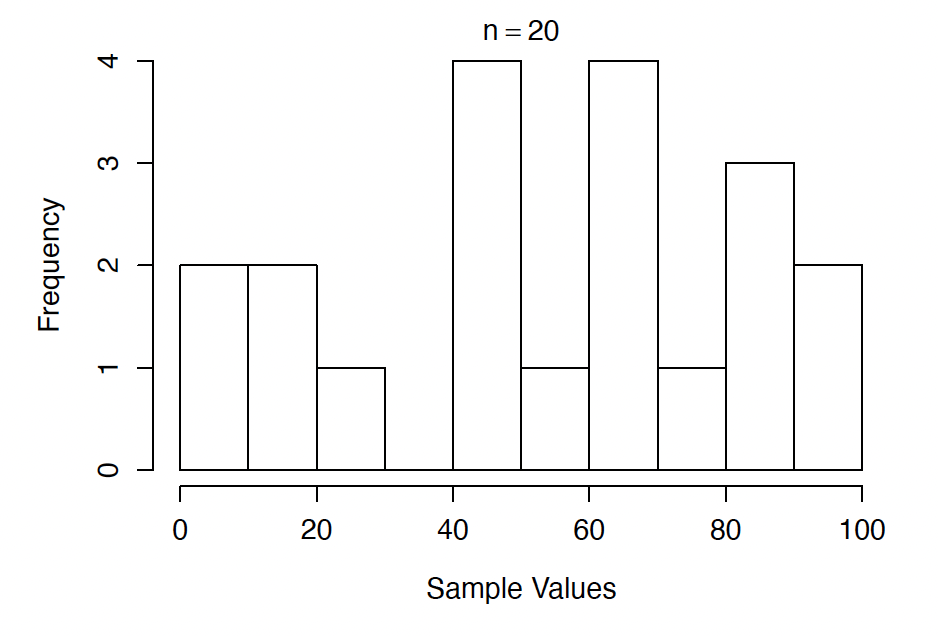
\includegraphics[width=8cm]{histo.png}
		\begin{tabular}{cc}
		\toprule
		Sample Mean& 54.1762\\
		Sample Variance&924.8788 \\
		\bottomrule
	\end{tabular}
\end{frame}

\begin{frame}{Histogram}
	
%\begin{itemize}[label={\color{blue}$\blacktriangleright$}]
%\item Why does the histogram not look more like a uniform distribution?
%\end{{itemize}
\begin{itemize}[label={\color{blue}$\blacktriangleright$}]
	\item Why does the histogram not look more like a uniform distribution?
\end{itemize}
	
	\centering
	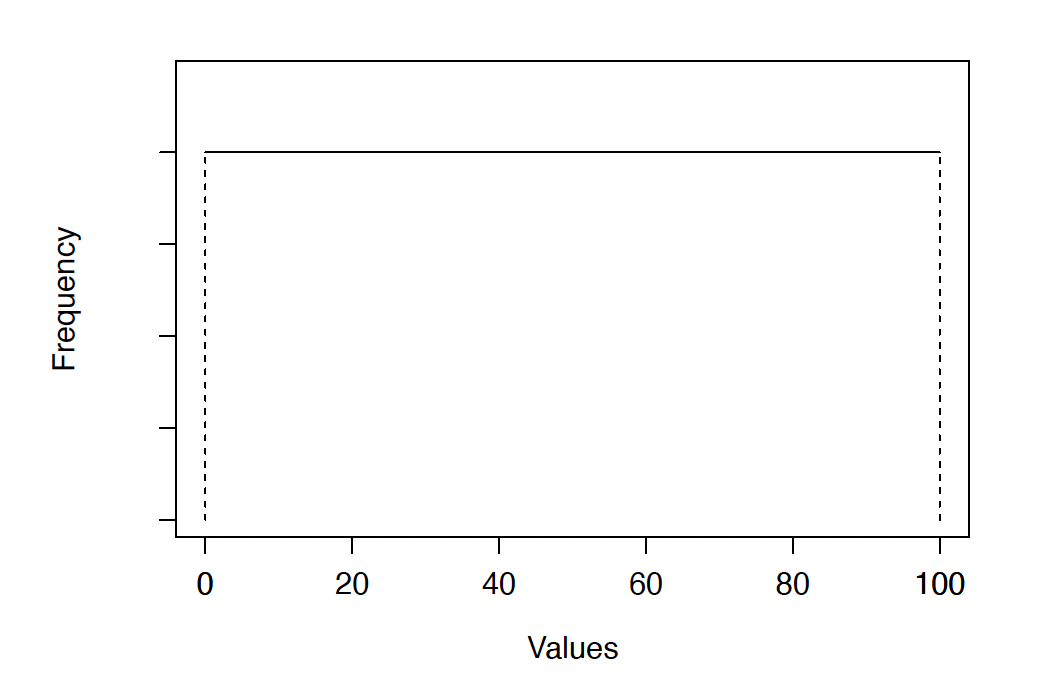
\includegraphics[width=8cm]{histo2.png}
	
\end{frame}

\begin{frame}
	\frametitle{Sample Statistics}
	
	\begin{itemize}[label={\color{blue}$\blacktriangleright$}]
		\item Why is the sample mean not equal (or close) to:
		
		\[E(X) = \frac{a + b}{2} = \frac{0 + 100}{2} = 50?\]
		
		\item Why is the sample variance not equal (or close) to:
		
		\[V(X) = \frac{(b - a)^2}{12} = \frac{(100 - 0)^2}{12} = 833.3333?\]
	\end{itemize}
	
\end{frame}

\begin{frame}[fragile]
	\frametitle{$n = 1000$}
	
	\begin{verbatim}
		> n <- 1000  # Sample size.
		> unif.data <- runif(n,min=0,max=100)
		> hist(unif.data,breaks=10)
		> mean(unif.data)
		[1] 50.71992
		> var(unif.data)
		[1] 802.7182
	\end{verbatim}
	
\end{frame}

\begin{frame}{$n=1000$}
	
	\centering
	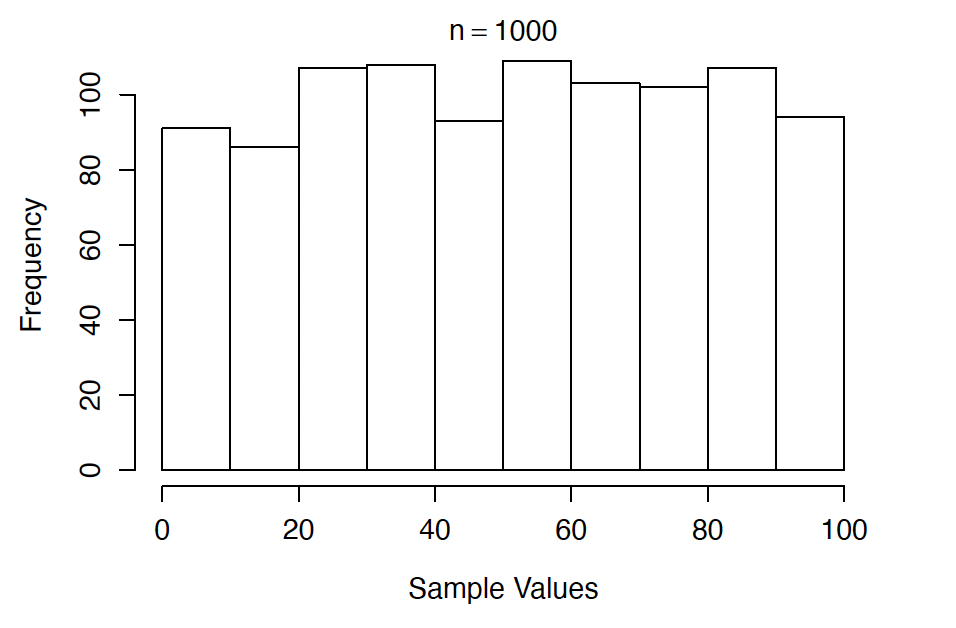
\includegraphics[width=8cm]{histo3.png}
	\begin{tabular}{cc}
		\toprule
		Sample Mean& 50.7199\\
		Sample Variance&802.7182 \\
		\bottomrule
	\end{tabular}
\end{frame}
\begin{frame}[fragile]
	\frametitle{$n = 20000$}

	
	\begin{verbatim}
		> n <- 20000  # Sample size.
		> unif.data <- runif(n,min=0,max=100)
		> hist(unif.data,breaks=10)
		> mean(unif.data)
		[1] 49.93417
		> var(unif.data)
		[1] 833.4439
	\end{verbatim}
	
\end{frame}
\begin{frame}{$n=2000$}
	
	\centering
	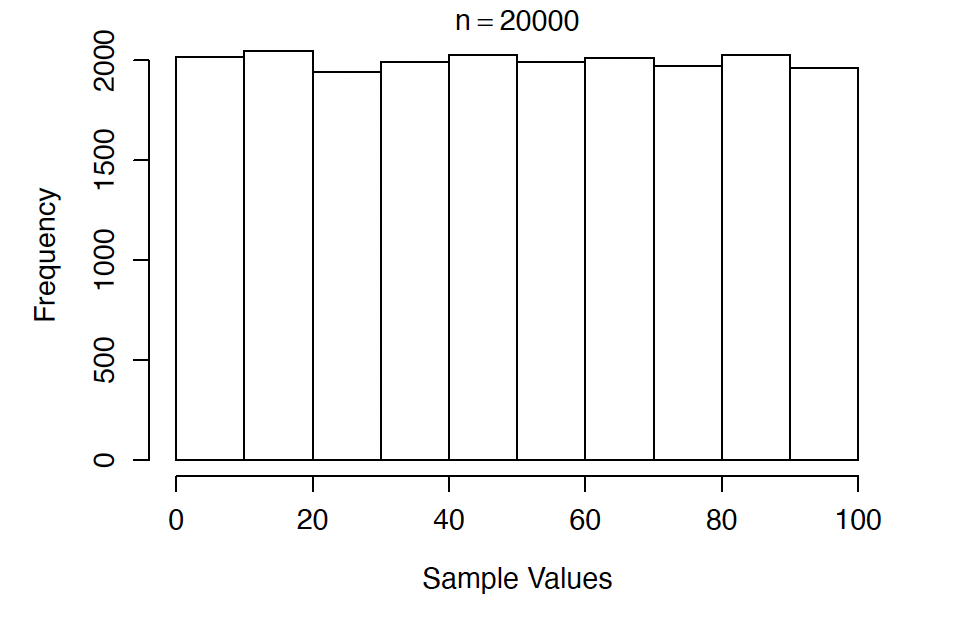
\includegraphics[width=8cm]{histo4.png}
	\begin{tabular}{cc}
		\toprule
		Sample Mean& 49.9342\\
		Sample Variance&833.4439 \\
		\bottomrule
	\end{tabular}
\end{frame}

\begin{frame}{Summary}
	\begin{itemize}[label={\color{blue}$\blacktriangleright$}]
		\item As $n$ increases, the histogram of the sample values begins to look more like the distribution of the population (i.e., the uniform distribution).
		\item {\color{red}As $n$ increases, the sample mean and the sample variance converge towards the population mean and population variance, respectively.}
	\end{itemize}
\end{frame}
\begin{frame}
	\frametitle{Another Experiment}
	\begin{itemize}[label={\color{blue}$\blacktriangleright$}]
		\item Let's now redo the previous experiment, but this time generating multiple samples at the same time.
		\item We'll examine the sample means of the samples and analyze their characteristics (e.g., histograms and sample statistics).
		\item See what happens when we change vary the sample size $n$.
	\end{itemize}
	
\end{frame}
\begin{frame}
	\frametitle{Another Experiment}
	
\centering
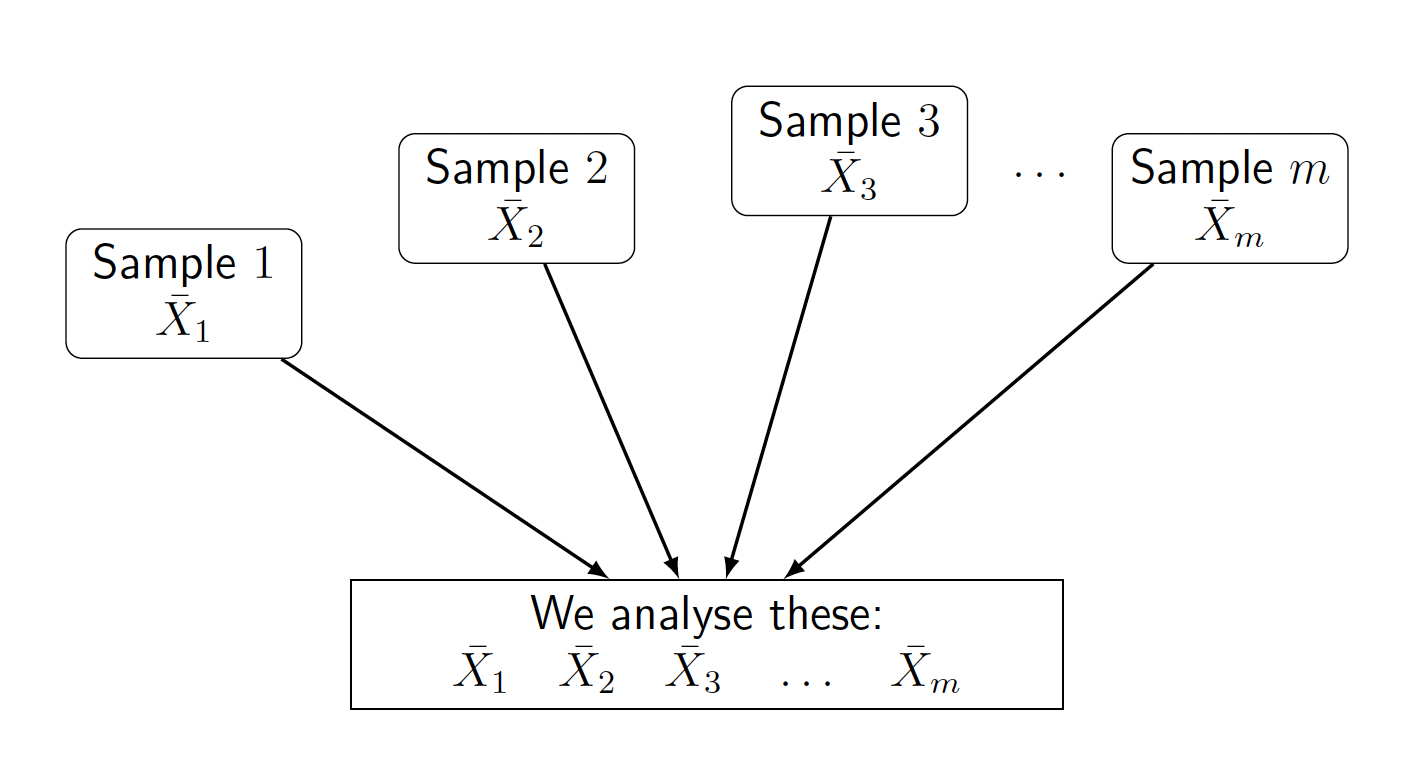
\includegraphics[width=12cm]{anther.png}
	
\end{frame}
\begin{frame}{Histogram for Sample Means}
	$n=20$ is sample size, $m=1000$ is number of samples
	\centering
	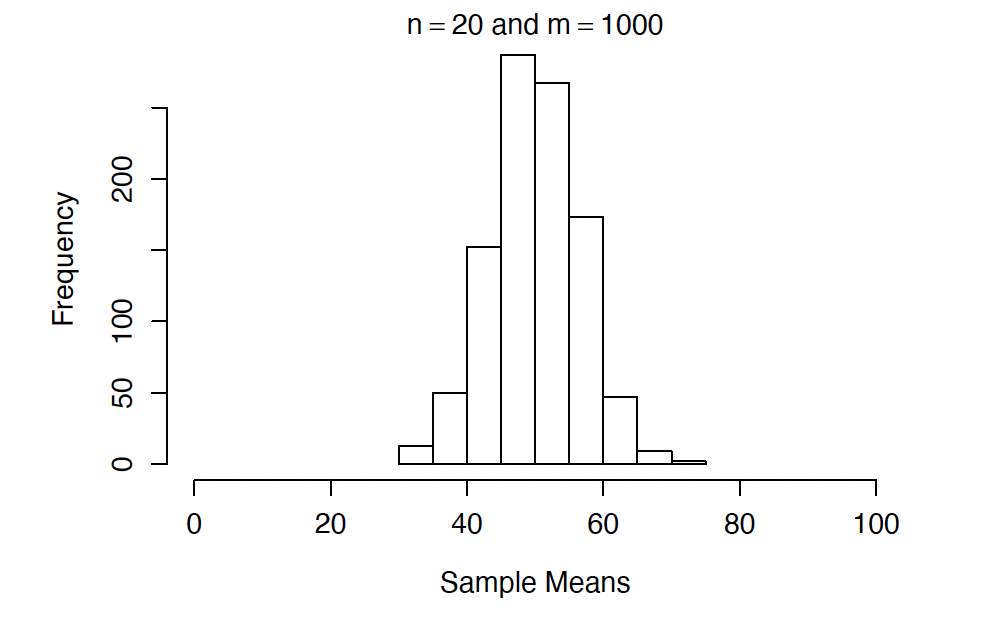
\includegraphics[width=9cm]{histo5.png}
	\begin{tabular}{cc}
		\toprule
		Mean of Sample Means& 49.9882\\
		Variance of Sample Means&42.8857\\
		\bottomrule
	\end{tabular}
\end{frame}
\begin{frame}
	\frametitle{Summary}
	\begin{itemize}[label={\color{blue}$\blacktriangleright$}]
		\item The sampling distribution of the sample mean looks like a normal distribution!
		\item This phenomenon, called the {\bf Central Limit Theorem}, will occur regardless of the underlying distribution of the population (in this case, a uniform distribution).
		\item The mean of the sampling distribution of the sample mean is equal to $\mu$, the population mean of $X$.
	\end{itemize}
	
\end{frame}
\begin{frame}
	\frametitle{Mean of the Sample Mean}
	
	\begin{itemize}[label={\color{blue}$\blacktriangleright$}]
		\item Let $X_1, X_2, \ldots, X_n$ denote our random sample.
		
		\item We know that the $X_i$ are independent and that 
		$E(X_i) = \mu$ and $V(X_i) = \sigma^2$ for each $i$.
		
		\item The sample mean is given by:
		
		\[ \bar{X} = \frac{1}{n}(X_1 + \ldots + X_n) \]
		
		\item Therefore, we can use the laws of expected value to calculate $\mu_{\bar{X}} = E(\bar{X})$.
	\end{itemize}
	
\end{frame}
\begin{frame}
	\frametitle{Mean of the Sample Mean}
	
	\begin{align*}
		\mu_{\bar{X}} &= E(\bar{X}) = E\left(\frac{1}{n}(X_1 + \ldots + X_n)\right) \\
		&= \frac{1}{n}E(X_1 + \ldots + X_n) \\
		&= \frac{1}{n}(E(X_1) + \ldots + E(X_n)) \\
		&= \frac{1}{n}(\mu + \ldots + \mu) \\
		&= \frac{1}{n} \times n\mu \\
		&= \mu
	\end{align*}
	
\end{frame}
\begin{frame}
	\frametitle{$n=100$ and $m=100$}
	
	\begin{itemize}[label={\color{blue}$\blacktriangleright$}]
		\item Let's see what happens when we increase the sample size (i.e., the number of observations in each sample) from $n=20$ to $n=100$.
		
		\item We'll leave the number of samples to be $m = 1000$, as before.

	\end{itemize}
	
\end{frame}

\begin{frame}{Histogram for Sample Means}
	$n=100$ is sample size, $m=1000$ is number of samples
	\centering
	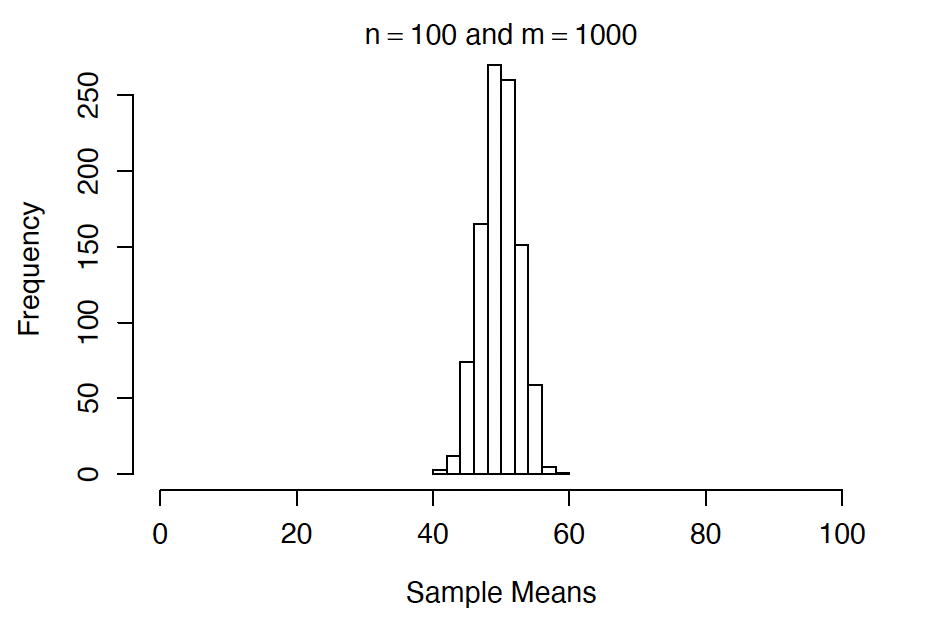
\includegraphics[width=8cm]{histo6.png}
	\begin{tabular}{cc}
		\toprule
		Mean of Sample Means& 49.8028\\
		Variance of Sample Means&7.5377\\
		\bottomrule
	\end{tabular}
\end{frame}
\begin{frame}
	\frametitle{Comparison of $n=20$ to $n=100$}
	\begin{columns}
		\column{0.48\textwidth}
		\begin{figure}
			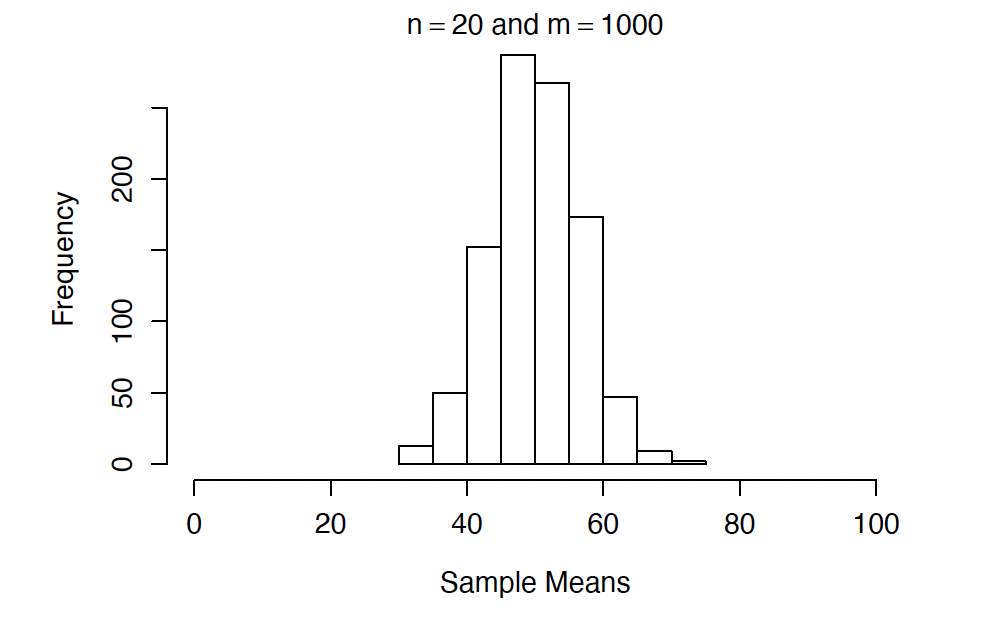
\includegraphics[width=5.2cm]{histo5.png}
		\end{figure}

%	\begin{tabular}{cc}
%	\toprule
%	Sample Mean& 49.9882\\
%	Variance of Sample Means&42.8857\\
%	\bottomrule
%\end{tabular}

		
		\column{0.48\textwidth}
		\begin{figure}
			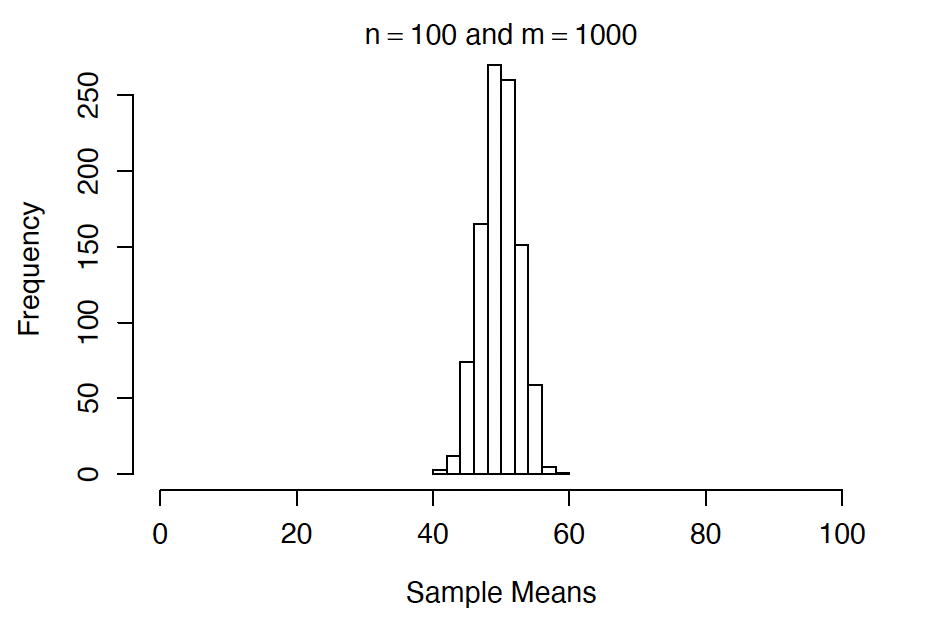
\includegraphics[width=5cm]{histo6.png}
		\end{figure}
%	\begin{tabular}{cc}
%	\toprule
%	Sample Mean& 49.8028\\
%	Variance of Sample Means&7.5377\\
%	\bottomrule
%\end{tabular}

	\end{columns}
	\centering
		\begin{tabular}{ccc}
		\toprule
		&$n=20$&$n=100$\\
		\midrule
		Mean of Sample Means& 49.9882&49.8028\\
		Variance of Sample Means&42.8857&7.5377\\
		\bottomrule
	\end{tabular}
\end{frame}
\begin{frame}
	\frametitle{Summary}
	
	\begin{itemize}[label={\color{blue}$\blacktriangleright$}]
		\item The sample variance of the sample means gets smaller as the sample size $n$ increases!
		
		\item The variance of the sampling distribution of the sample mean is equal to $\frac{\sigma^2}{n}$, the population variance of $X$ divided by $n$.
		
		\item The standard deviation of the sampling distribution of the sample mean is equal to $\frac{\sigma}{\sqrt{n}}$.
		
		\item Note: The standard deviation of a sample statistic is called the \textbf{standard error (SE)} of the statistic.
	\end{itemize}
	
\end{frame}
\begin{frame}
	\frametitle{Variance of the Sample Mean}
	
	\begin{align*}
		\sigma^2_{\bar{X}} &= V(\bar{X}) = V\left(\frac{1}{n}(X_1 + \ldots + X_n)\right) \\[0.5em]
		&= \frac{1}{n^2}V(X_1 + \ldots + X_n) \\[0.5em]
		&= \frac{1}{n^2}(V(X_1) + \ldots + V(X_n)) \\[0.5em]
		&= \frac{1}{n^2}(\sigma^2 + \ldots + \sigma^2) \\[0.5em]
		&= \frac{1}{n^2} \times n\sigma^2 \\[0.5em]
		&= \frac{\sigma^2}{n}
	\end{align*}
	
\end{frame}
\begin{frame}
	\frametitle{Central Limit Theorem}
	
	\begin{itemize}[label={\color{blue}$\blacktriangleright$}]
		\item Let $X_1, \ldots, X_n$ be a random sample from a population with mean $\mu$ and variance $\sigma^2$ (i.e., the $X_i$'s are independent and $E(X_i) = \mu$ and $V(X_i) = \sigma^2$ for $i = 1, \ldots, n$). Then:
		
		\vspace{0.5em}
		
		\[\bar{X} \sim N\left(\mu_{\bar{X}} = \mu, \sigma^2_{\bar{X}} = \frac{\sigma^2}{n}\right) \quad \text{as} \quad n \to \infty\]
		
		\vspace{0.5em}
		
		\item Which means if we standardize:
		
		\vspace{0.5em}
		
		\[\frac{\bar{X} - \mu}{\sigma / \sqrt{n}} = Z \sim N(0, 1) \quad \text{as} \quad n \to \infty\]
	\end{itemize}
	
\end{frame}
\begin{frame}
	\frametitle{How Large Should $n$ Be?}
	
	\begin{itemize}[label={\color{blue}$\blacktriangleright$}]
		\item Generally, it depends on the population distribution of $X$.
		\begin{itemize}[label={\color{blue}$\blacktriangleright$}]
			\item If $X$ has a normal distribution, then the sample mean has a normal distribution for \textit{all} sample sizes.
			\item If $X$ has a distribution that is close to normal, the approximation is good for small sample sizes (e.g., $n \approx 20$).
			\item If $X$ has a distribution that is far from normal, the approximation requires larger sample sizes (e.g., $n > 50$).
		\end{itemize}
	\end{itemize}
	
\end{frame}

\begin{frame}
	\frametitle{Example 1}
	
	\begin{itemize}[label={\color{blue}$\blacktriangleright$}]
		\item Consider the marks of all students who took an economics test. If marks are normally distributed, with mean equal to 72 and standard deviation equal to 9, find:
			\end{itemize}
		
		(a) The probability that any one student will have a mark over 78.
		
		(b) The probability that a sample of 10 students will have an average mark over 78.

	
\end{frame}

\begin{frame}
	\frametitle{Solution - Part (a)}
	
	\begin{itemize}[label={\color{blue}$\blacktriangleright$}]
		\item Let $X$ be the mark of a randomly selected student.
		\item Then $X \sim N(\mu = 72, \sigma^2 = 9^2)$.
	\end{itemize}
	
	\vspace{0.5em}
	
	\begin{align*}
		P(X > 78) &= P\left(\frac{X - \mu}{\sigma} > \frac{78 - 72}{9}\right) \\[0.5em]
		&= P(Z > 0.67) \\[0.5em]
		&= 1 - P(Z < 0.67) \\[0.5em]
		&= 1 - 0.7486 \\[0.5em]
		&= 0.2514
	\end{align*}
	
\end{frame}
\begin{frame}{Solution - Part (a)}
	
	\centering
	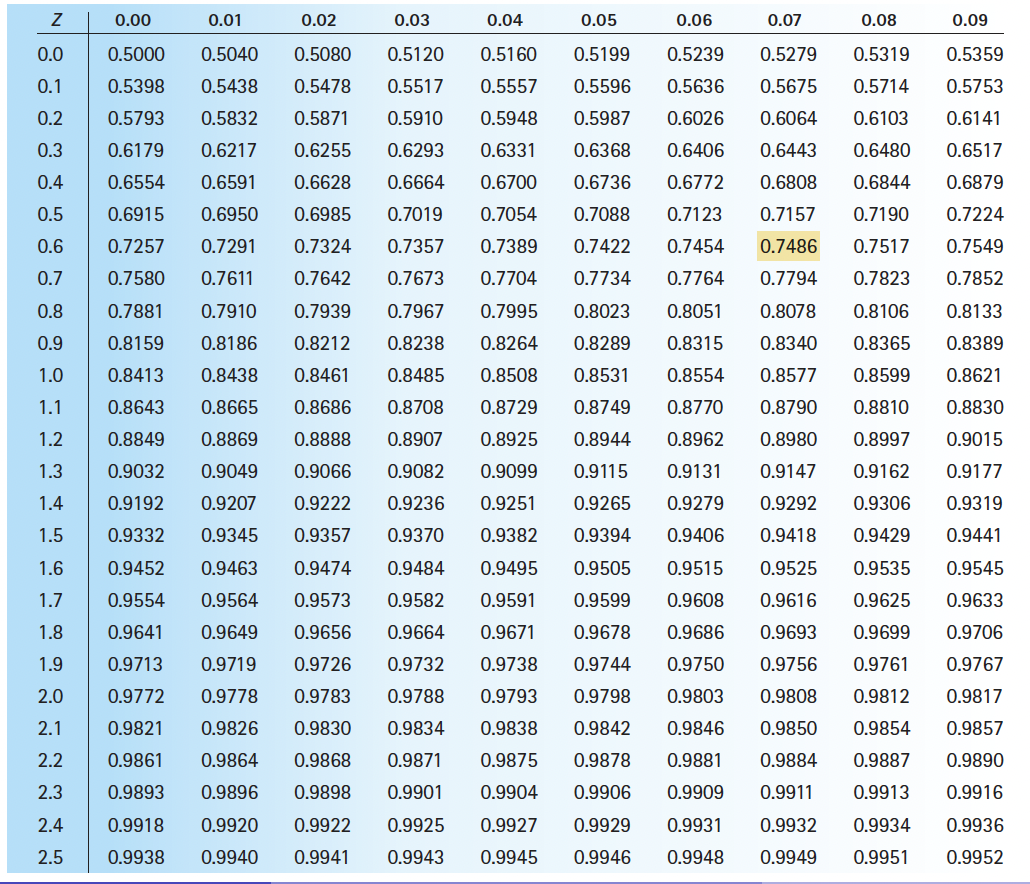
\includegraphics[width=10cm]{ztable.png}

\end{frame}

\begin{frame}
	\frametitle{Solution - Part (b)}
	
	\begin{itemize}[label={\color{blue}$\blacktriangleright$}]
		\item Let $\bar{X}$ be the average mark of the sample of 10 students.
		\item By CLT, $\bar{X} \sim N\left(\mu_{\bar{X}} = \mu = 72, \sigma^2_{\bar{X}} = \frac{\sigma^2}{n} = \frac{9^2}{10}\right)$.
	\end{itemize}
	
	\vspace{0.5em}
	
	\begin{align*}
		P(\bar{X} > 78) &= P\left(\frac{\bar{X} - \mu_{\bar{X}}}{\sigma_{\bar{X}}} > \frac{78 - 72}{\frac{9}{\sqrt{10}}}\right) \\[0.5em]
		&= P(Z > 2.11) \\[0.5em]
		&= 1 - P(Z < 2.11) \\[0.5em]
		&= 1 - 0.9826 \\[0.5em]
		&= 0.0174
	\end{align*}
	
\end{frame}
\begin{frame}{Solution - Part (b)}
	
	\centering
	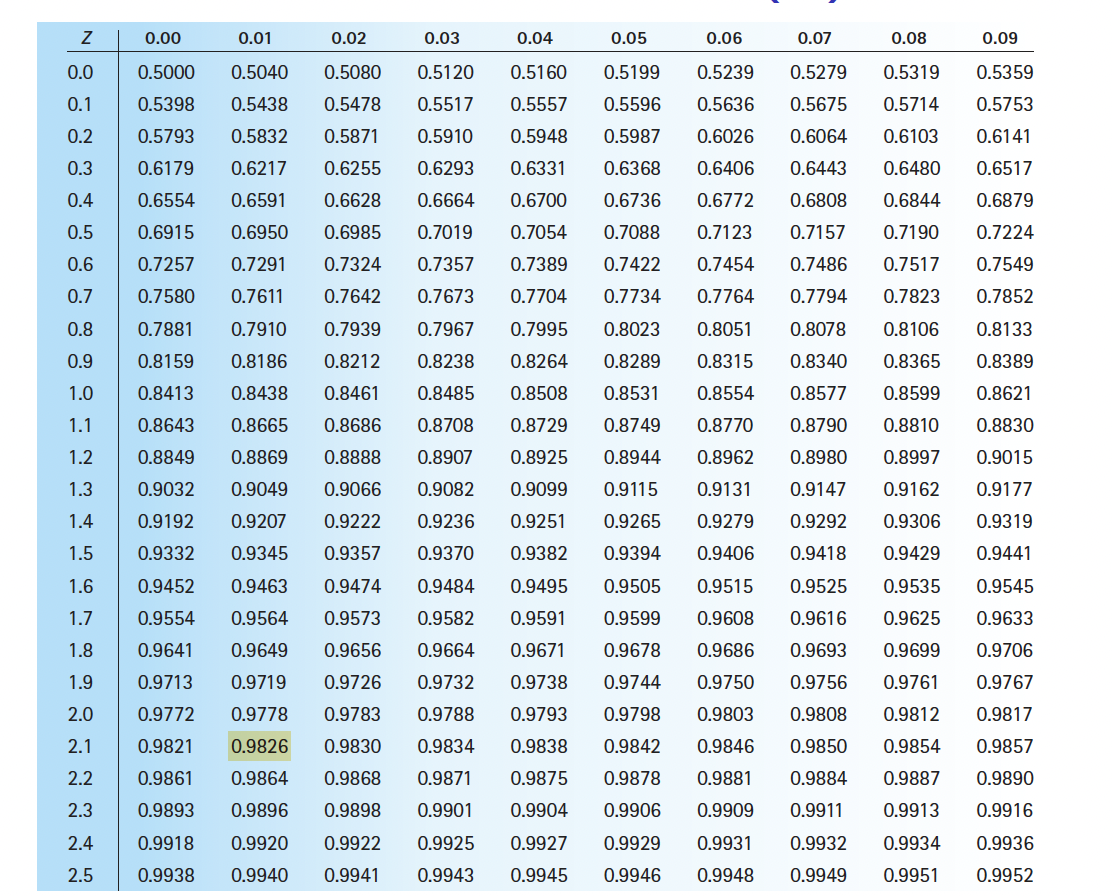
\includegraphics[width=10cm]{ztable2.png}
	
\end{frame}

\begin{frame}
	\frametitle{Comparing Parts (a) and (b)}
	
	\begin{itemize}[label={\color{blue}$\blacktriangleright$}]
		\item Why does the probability drop from 25.14\% to 1.74\%?
		\begin{itemize}[label={\color{blue}$\blacktriangleright$}]
			\item The standard deviation of sample means (or the \textit{standard error}) is always smaller than the standard deviation of single observations.
		\end{itemize}
		
		\item Interpretation:
		\begin{itemize}[label={\color{blue}$\blacktriangleright$}]
			\item Sample means have less variability than single observations.
		\end{itemize}
		
		\item E.g., much more likely to find an individual who is very smart, than a random sample of 10 students who are all very smart.
	\end{itemize}
	
\end{frame}

\end{document}